\documentclass{WTC2027}
\usepackage[T1]{fontenc}
\usepackage{textcomp}
\usepackage{newtxtext}
\usepackage{newtxmath}
\usepackage{booktabs}
\usepackage{multirow}
\usepackage{graphicx}
\usepackage{tikz}
\usetikzlibrary{arrows.meta,positioning,fit,backgrounds,calc}
\definecolor{wffield}{HTML}{DCEAF7}
\definecolor{wfdensity}{HTML}{E3F0E5}
\definecolor{wfpipeline}{HTML}{F8E6D2}
\definecolor{wfdecision}{HTML}{F5EDC8}
\definecolor{wfcheck}{HTML}{E9ECEF}
\definecolor{wfink}{HTML}{263746}
\usepackage{amsmath}
\usepackage{array}
\usepackage{tabularx}
\usepackage[style=authoryear,backend=biber,sorting=nyt,doi=false,isbn=false,eprint=false,autopunct=false,giveninits=true,uniquename=init,uniquelist=false,maxcitenames=2,mincitenames=1,maxbibnames=99]{biblatex}
\urlstyle{same}
\graphicspath{{images/}}
\newcommand{\labelledpanel}[3][]{%
\begin{tikzpicture}
\node[anchor=south west,inner sep=0,outer sep=0] (panel) at (0,0) {\includegraphics[height=38mm]{#3}};
\node[anchor=north west,fill=white,fill opacity=0.72,text opacity=1,
      inner xsep=3pt,inner ysep=2pt,font=\bfseries\fontsize{9}{10}\selectfont]
      at ([xshift=0.5mm,yshift=-0.5mm]panel.north west) {(#2)};
#1
\end{tikzpicture}%
}
\addbibresource{references.bib}
\DeclareLabeldate[online]{\field{date}\field{year}\literal{nodate}}
\DefineBibliographyStrings{english}{and={\&},}
% Author-date bibliography, with explicit surname/initial separators.
\DeclareNameAlias{sortname}{family-given}
\renewcommand*{\bibinitperiod}{.}
\renewcommand*{\revsdnamepunct}{,\space}
\DeclareDelimFormat[bib,biblist]{multinamedelim}{,\space}
\DeclareDelimFormat[bib,biblist]{finalnamedelim}{\space\&\space}
% Match the WTC website examples while retaining the official authoryear framework.
% Initials distinguish T. Wang and Y. Wang in citations from the same year.
\DeclareDelimFormat{finalnamedelim}{\addspace\&\space}
\DeclareDelimFormat[bib,biblist]{nameyeardelim}{\addspace}
\renewbibmacro*{date+extradate}{\printlabeldateextra}
\DeclareFieldFormat[article,inproceedings,misc]{title}{#1}
\DeclareFieldFormat[article]{pages}{#1}
\setlength{\bibhang}{4mm}
\DeclareBibliographyDriver{article}{%
  \usebibmacro{bibindex}\usebibmacro{begentry}%
  \usebibmacro{author/translator+others}%
  \setunit{.\space}\printfield{title}%
  \setunit{.\space}\newblock\printfield{journaltitle}%
  \setunit{\addspace}\printfield{volume}%
  \printfield[parens]{number}%
  \setunit{:\space}\printfield{pages}%
  \usebibmacro{finentry}}
\renewbibmacro*{in:}{\printtext{In\space}}
\renewcommand{\bibfont}{\fontsize{10pt}{11pt}\selectfont}
\AtBeginDocument{\setlength{\bibitemsep}{0pt}\setlength{\baselineskip}{12pt}}
\raggedbottom

\begin{document}

% Approved author order retained; initials follow the official template.
\author{Z.~Yao\textsuperscript{1}, Y.~Zhou\textsuperscript{2,*},
L.~Huang\textsuperscript{3,*}, S.~Liu\textsuperscript{1},
Y.~Wang\textsuperscript{1}, Z.~Zhang\textsuperscript{1},
Y.~Wang\textsuperscript{2}, H.~Fei\textsuperscript{2},
B.~Yu\textsuperscript{4}, J.~Lei\textsuperscript{3},
T.~Song\textsuperscript{3}, Z.~Zhao\textsuperscript{3},
Z.~Xiong\textsuperscript{3}, K.~Li\textsuperscript{3},
\& Z.~Zhang\textsuperscript{5}}
\aff{\textsuperscript{1}University of Science and Technology of China, Hefei, China\\
\textsuperscript{2}Jianwei Scientific Instruments (Anhui) Technology Co., Ltd., Hefei, China\\
\textsuperscript{3}Shenzhen Metro Group Co., Ltd., Shenzhen, China\\
\textsuperscript{4}Jianwei Geophysical Exploration (Shenzhen) Technology Co., Ltd., Shenzhen, China\\
\textsuperscript{5}China Railway No.8 Engineering Group Co., Ltd., Chengdu, China\\[3pt]
\textsuperscript{*}Corresponding authors: Yong Zhou (\nolinkurl{zhouyong@jwky.com});\\
Liping Huang (\nolinkurl{huanglp@shenzhenmc.com}).}

\abstract{Uncertain ground conditions and buried utilities complicate shield tunnelling, while boreholes and surface investigations may provide incomplete coverage in dense urban settings. Cosmic-ray muography offers a passive means of investigating subsurface density, but field deployment requires instrumentation that can operate under construction vibration, elevated temperature, high humidity and restricted access. This paper presents a field-deployable three-layer Micromegas muography system and two applications on Shenzhen Metro Line~22. The system incorporates environmental control, pneumatic vibration isolation, a low-consumption gas supply, condition monitoring and integrated data acquisition for both mobile and stationary measurements. Aboard tunnel boring machines, it operated at depths of about 15--30~m over 1371 rings; on the right line, acquisition availability was 85.2\%, or 97.2\% excluding external power and network interruptions, and platform vibration was not detected inside the isolated enclosure. Measurements at two shield positions were combined with tunnel geometry and borehole stratigraphy to reconstruct density corrections relative to a geological reference model, indicating a possible low-density region above and to one side of the tunnel. In a separate static investigation, observations from four detector positions were processed using position-specific U-Net models and multi-view geometry to estimate a candidate buried-pipeline axis. The result was supplied as a spatial constraint for construction planning, but was not independently confirmed. The deployments demonstrate the field feasibility and decision-support potential of muography for subsurface investigation during tunnel construction, while highlighting the need for matched reference measurements, uncertainty quantification and independent validation.}

\keywords{muography; shield tunnelling; density reconstruction; pipeline localisation}

\chapter{Subsurface imaging in shield tunnelling and pipeline localisation via a robust cosmic-ray muography system: a field study}

\section{INTRODUCTION}
Uncertain ground conditions and buried utilities can interrupt shield advance and threaten surrounding infrastructure. Boreholes provide direct but spatially discrete geological information, while urban access restrictions and ongoing construction can constrain surface investigations. Measurements acquired from within a tunnel can therefore complement conventional surveys by providing directional information about the ground surrounding the excavation.

Cosmic-ray muography exploits atmospheric muons that retain sufficient energy to reach an underground detector after traversing soil and rock. The transmission approach used here measures the directional flux remaining after passage through the target \autocite{procureur2018}. Comparing the underground flux with an open-sky reference gives the density integrated along each muon path, and views from several directions and positions can be combined with tunnel geometry and geological information to locate density variations. The method is passive and requires neither an artificial radiation source nor access to the target.

Previous underground studies have reconstructed overburden density and rock--air interfaces from multiple detector locations \autocite{guardincerri2017}, identified concealed construction shafts and a subsequently confirmed overburden void in a railway tunnel \autocite{thompson2020}, and detected structural changes along a subway station and tunnel \autocite{mao2023}. These studies establish the potential of tunnel-based measurements, but sustained deployment during active shield construction introduces additional instrumentation and operational requirements.

Mounting a detector on an operating tunnel boring machine (TBM) exposes it to vibration, heat and humidity in a confined space with limited maintenance access, and the observation geometry changes as the shield advances. A stationary investigation instead requires the instrument to be repositioned accurately to combine several views of a fixed target.

This paper presents a field-deployable three-layer Micromegas muography platform supporting both dynamic TBM-mounted measurements and stationary multi-position tunnel investigations. The contributions are: (1) a system designed for construction conditions; (2) an assessment of sustained operation on Shenzhen Metro Line~22; and (3) two field demonstrations, comprising TBM-mounted ground-density imaging and a four-position investigation of a suspected buried pipeline. 

\section{MUOGRAPHY SYSTEM AND FIELD PERFORMANCE}
\subsection{Detector and tracking principle}
The tracking unit comprises three thermally bonded Micromegas layers, each with a $40\times40$~cm$^2$ sensitive area and separated by approximately 15~cm \autocite{feng2021thermal}. Orthogonal strip readouts provide two-dimensional hit positions with an effective pitch of 1.6~mm, allowing each muon trajectory to be reconstructed by fitting hits across the three layers. Compact front-end cards digitise the signals, while a central data acquisition board forms inter-layer coincidences and aggregates the events. Optical fibres connect the front-end electronics to the acquisition board, and data are transferred to the control computer via USB~3.0 \autocite{wang2025readout,liu2025backend}. Table~\ref{tab:specs} summarises the main specifications of the deployed system.

\begin{table}[htbp]
\caption{Main specifications of the muography system.}
\label{tab:specs}\centering
\fontsize{10pt}{12pt}\selectfont
\renewcommand{\arraystretch}{1.12}
\setlength{\tabcolsep}{5pt}
\begin{tabularx}{\textwidth}{@{}l>{\raggedright\arraybackslash}Xl>{\raggedright\arraybackslash}X@{}}
\toprule
Item & Value & Item & Value\\
\midrule
Detector & Micromegas, 3 layers & Main enclosure & $700\times450\times800$~mm, 85~kg\\
Sensitive area & $400\times400$~mm per layer & Gas enclosure & $350\times330\times750$~mm, 25~kg\\
Layer spacing & 150~mm (300~mm baseline) & Protection & IP56\\
Readout & X--Y strips, 1.6~mm pitch & Power & 220~V AC, 800~W\\
Layer efficiency & $>95\%$ (nominal) & Data interfaces & Ethernet, RS485\\
Angular resolution & $0.3^\circ$ (nominal) & Inclination & $35^\circ$, adjustable\\
Max.\ event rate & 3~kHz & Monitoring & Temperature, humidity, inclination, vibration\\
\bottomrule
\end{tabularx}
\end{table}

\subsection{Field-compatible system design}
Shield tunnelling exposes the instrument to heat and humidity, machine vibration, a continuously changing observation geometry and limited access for maintenance. The IP56 main enclosure integrates the detectors, readout electronics, power supplies and a sealed air-conditioning unit that controls internal temperature and humidity. For TBM-mounted operation, four pneumatic isolators separate the inclined detector frame from the shield support platform, and vibration sensors on the platform and inside the enclosure record the vibration on each side of the isolators. An inclinometer records the detector inclination so that each measurement can be associated with its observation geometry. A dedicated gas-control subsystem in a separate enclosure supplies the argon--carbon-dioxide mixture with much lower consumption than laboratory flow-gas operation; a single 8~L cylinder at 10~MPa sustained approximately three months of field operation, which set the routine maintenance interval. Detector status, environmental and vibration data are available over Ethernet or RS485 for remote monitoring. Figure~\ref{fig:installation} shows the enclosure design with dimensions (a), internal arrangement (b) and installation on the TBM (c).

\subsection{Field deployment and operational performance}
The system operated at depths of approximately 15--30~m in the Guihua Station--Songyuanxia Station interval from 6~November~2025 to 27~July~2026, covering 1371 rings (428 on the left line and 943 on the right). It was installed approximately 5~m behind the cutterhead on the left line and 15~m behind it on the right. Detector positions and orientations were associated with the corresponding ring records for subsequent analysis. Monitored enclosure temperatures remained below $40\,^{\circ}$C and relative humidity below 70\%.

On the right line, normal acquisition totalled 2965.5~h, or 85.2\% of the 3480.0~h monitoring record. The availability was 97.2\% after 401.5~h of external power loss and 28.3~h of network interruption were excluded. The remaining 84.7~h comprised system maintenance.

Figure~\ref{fig:vibration} shows a 34~h record from 14--15 February 2026. Platform vibration began at 19:15 and continued for the remaining 14.7~h, with a typical peak particle velocity (PPV, vector sum of three axes) of 0.21~mm/s, 99\% of readings below 2.8~mm/s and a maximum of 3.7~mm/s. No vibration was recorded inside the enclosure. The reconstructed three-layer track rate was 13.54~min$^{-1}$ in the 19.2~h before platform vibration began and 13.34~min$^{-1}$ during it, a difference of about 1.2 standard errors, and its 5-min fluctuations (1.46 and 1.60~min$^{-1}$) were consistent with counting statistics alone (about 1.6~min$^{-1}$). Within this record, platform vibration was therefore not transmitted to the detectors at a detectable level, and detector operation was not measurably affected.


\begin{figure}[htbp]
\centering
\begin{minipage}[t]{0.38\textwidth}\centering
\labelledpanel{a}{figure_enclosure_design.png}
\end{minipage}\hfill
\begin{minipage}[t]{0.32\textwidth}\centering
\labelledpanel{b}{figure_system_interior.png}
\end{minipage}\hfill
\begin{minipage}[t]{0.27\textwidth}\centering
\labelledpanel[{\begin{scope}[x={(panel.south east)},y={(panel.north west)}]
\foreach \pos in {(0.241,0.235)} {
  \draw[white,line width=1.0pt] \pos circle[radius=2.0mm];
  \draw[yellow!85!orange,line width=0.55pt] \pos circle[radius=2.0mm];
}
\node[anchor=south west,fill=white,fill opacity=0.8,text opacity=1,
      inner sep=1.5pt,font=\fontsize{7}{8}\selectfont] (isolatorlabel)
      at (0.04,0.04) {Pneumatic isolator};
\draw[white,line width=1.0pt] (isolatorlabel.north) -- (0.241,0.1824);
\draw[yellow!85!orange,line width=0.5pt] (isolatorlabel.north) -- (0.241,0.1824);
\end{scope}}]{c}{figure_tbm_deployment.png}
\end{minipage}
\caption{Muography system: (a) enclosure and exterior design with dimensions; (b) photograph showing the internal structure; (c) deployment on the tunnel boring machine.}
\label{fig:installation}
\end{figure}

\begin{figure}[htbp]
\centering
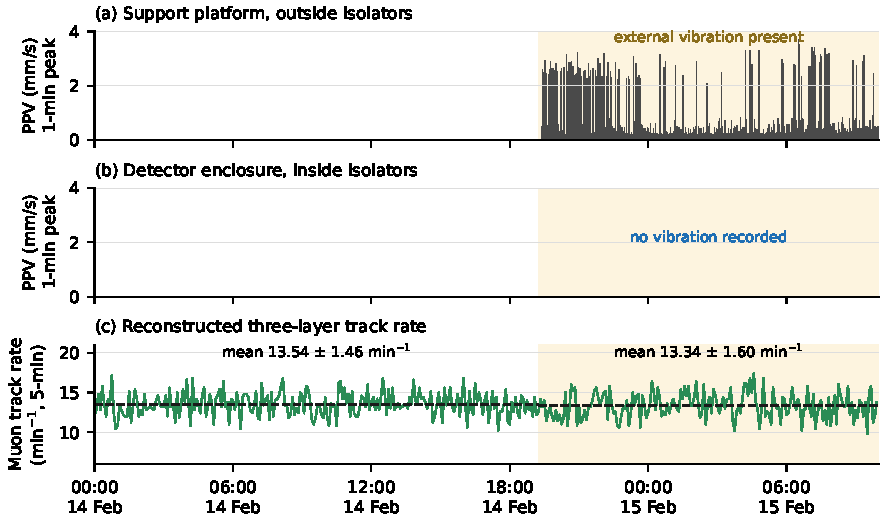
\includegraphics[width=\textwidth]{figure_vibration_isolation.pdf}
\caption{Vibration isolation during TBM operation, 14--15 February 2026 (Beijing time): (a) PPV on the shield support platform outside the isolators; (b) PPV inside the detector enclosure; (c) reconstructed three-layer muon track rate in 5-min windows, with period means (dashed). Shading marks the period with platform vibration.}
\label{fig:vibration}
\end{figure}

\section{FIELD DEMONSTRATION I: TBM-MOUNTED GROUND-DENSITY IMAGING}
\subsection{Engineering objective and site conditions}
The first demonstration examined whether measurements acquired during shield advance could identify density variations relative to the available geological model. Near the Fuzhou Avenue bridge, borehole stratigraphy provided a reference and two successive shield positions provided different viewing geometries. The result was intended for geological screening rather than confirmation of a specific feature.

\subsection{Measurements and reference model}
The primary dataset contains 5240 and 6840 selected underground tracks at rings 1672 and 1679, respectively. Underground exposures were 21.37 and 34.00~h. The corresponding open-sky reference measurements contained 457,255 selected tracks, with exposures of 20.97 and 66.52~h. The same detector hardware, track-reconstruction procedure and selection criteria were used for the open-sky and underground measurements.

In the survey frame, $Y$ is upward, $Z$ points towards decreasing ring number and $X$ is transverse, with the origin at ring 1672. The detector centres at the two rings were $(2,0,0)$ and $(2,0.27,-12.66)$~m, and the detector normal was inclined at $33.2^\circ$, varying within $\pm0.6^\circ$ during advance.

The reference model interpolates layer boundaries along the tunnel between 11 borehole control points and extends them uniformly across $X$. It comprises eight layers with assigned densities of 1.85--2.45~g\,cm$^{-3}$; the tunnel cavity and 0.4~m lining (outer diameter 8.8~m, density 2.4~g\,cm$^{-3}$) are modelled separately.

\subsection{Algorithm design}
The reconstruction compared measured and predicted directional counts, using the two underground observations, the open-sky reference, detector poses, tunnel geometry and the borehole model. For each trial density distribution on a 2~m grid, ray tracing calculated the material thickness traversed in each direction \autocite{siddon1985}. A muon spectrum \autocite{guan2015} and standard-rock ranges \autocite{groom2001} converted these thicknesses to expected counts, which a Poisson model compared with the measurements. A common factor of 0.53 normalised the two underground positions; it was estimated from background directions excluding known bridge piles and may also absorb differences between the sky and underground datasets.

Because only two viewing positions were available, the inversion was constrained by the geological reference and by spatial continuity. Departures from the borehole model were penalised more strongly near boreholes, while smoothing between neighbouring grid cells was reduced across interpreted layer boundaries. Sky rates and density corrections were estimated jointly within physical bounds, so the volume represents regularised corrections relative to the borehole model, rather than an independent absolute-density estimate.

Counts in 151 adaptive angular bins were fitted jointly for the main result and separately for each position; each single-position reconstruction was then used to predict the counts at the other position as a consistency check.

\subsection{Results and consistency checks}
Combining the two viewing geometries gives the density-correction distribution in Figure~\ref{fig:bridge-3d}; negative values indicate less density than the borehole model predicts. A possible low-density region appears above and to the negative-$X$ side of the tunnel. A positive correction near ring 1679 reaches $+0.57$~g\,cm$^{-3}$ at $(1,9,-9)$~m, a location directly sampled by that position.

A fixed set of voxels above the tunnel on its negative-$X$ side was selected from a preliminary joint reconstruction and retained for all fits. Its joint mean correction is $-0.36$~g\,cm$^{-3}$; separate fits to rings 1672 and 1679 give $-0.21$ and $-0.24$~g\,cm$^{-3}$, although their spatial distributions differ.

\begin{figure}[tbp]
\centering
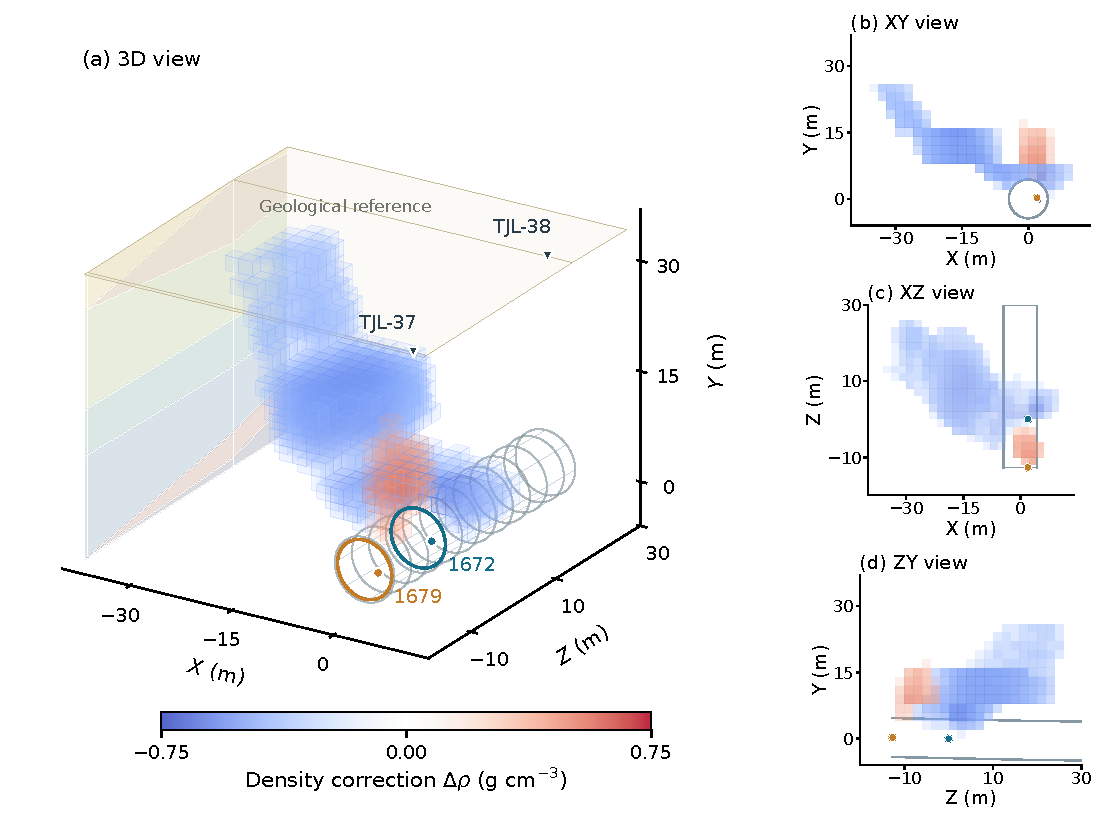
\includegraphics[width=0.80\textwidth]{figure_bridge_candidate_3d.pdf}
\caption{Joint density corrections relative to the borehole model: (a) three-dimensional rendering and (b--d) XY, XZ and ZY views. Only 2~m voxels with direct ray coverage and $|\Delta\rho|\geq0.35$~g\,cm$^{-3}$ are shown; transparency decreases with $|\Delta\rho|$.}
\label{fig:bridge-3d}
\end{figure}

In the cross-position check, each single-position reconstruction improved the prediction of the other position's counts (Poisson deviance reduced by 4--6\%), a modest improvement that is consistent with the negative regional means.

\subsection{Interpretation and limitations}
The result indicates a possible low-density region relative to the borehole model, not a confirmed void or material. Interpretation is limited by sparse borehole control, interpolated layer boundaries, non-simultaneous sky references, normalisation and regularisation. Because the comparison region was selected from a preliminary reconstruction, its mean is descriptive rather than an independent test statistic.

\section{FIELD DEMONSTRATION II: STATIC MULTI-POSITION PIPELINE INVESTIGATION}
\subsection{Engineering objective and survey arrangement}
Conventional detection methods had not located the pipeline at the position indicated in the original drawings, leaving uncertainty about its location relative to the planned tunnel alignment. The muography survey was therefore undertaken to investigate whether additional positional information could be obtained to inform pipeline-avoidance measures during shield advance.

The detector was deployed sequentially at four stationary positions within the tunnel, as shown in Figure~\ref{fig:pipeline-deployment}. Acquisition times at P0--P3 were 22.8, 21.7, 32.5 and 22.0~h, respectively. Tracks were binned into $36\times38$ directional maps, with 21,084--31,309 underground counts per position and 78,718 counts in the shared open-sky map.

Detector poses were surveyed in a frame centred on ring 252, with $X$ along the tunnel opposite to advance and $Z$ upward. The four positions spanned 11.3~m along the tunnel at the same height; the detector normal was inclined at 34--36$^\circ$ and rotated between $-77^\circ$ and $+35^\circ$ in azimuth to view the suspected crossing from different directions. The geometric model follows the construction drawings, with tunnel inner/outer radii of 2.75/3.10~m and ground at $Z=16.8$~m.

\begin{figure}[htbp]
\centering
\begin{tikzpicture}
\node[anchor=north west,inner sep=0] (A) at (0,0) {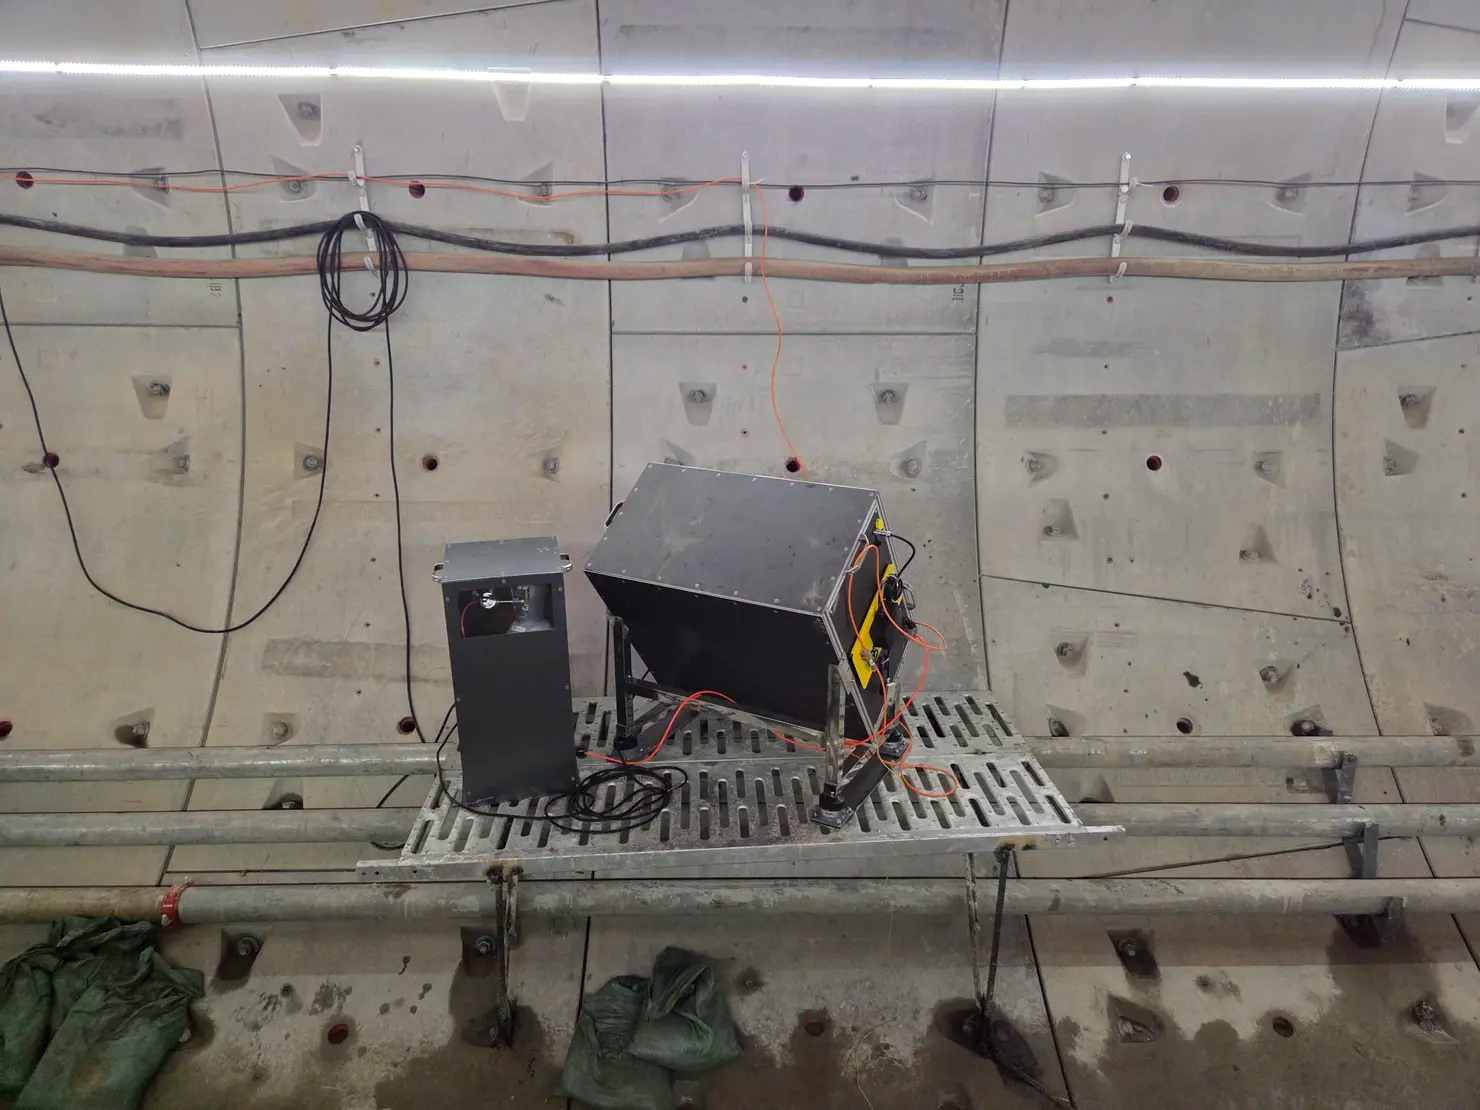
\includegraphics[width=0.244\textwidth]{pipeline_field_p0.png}};
\node[anchor=north west,inner sep=0] (B) at ([xshift=1mm]A.north east) {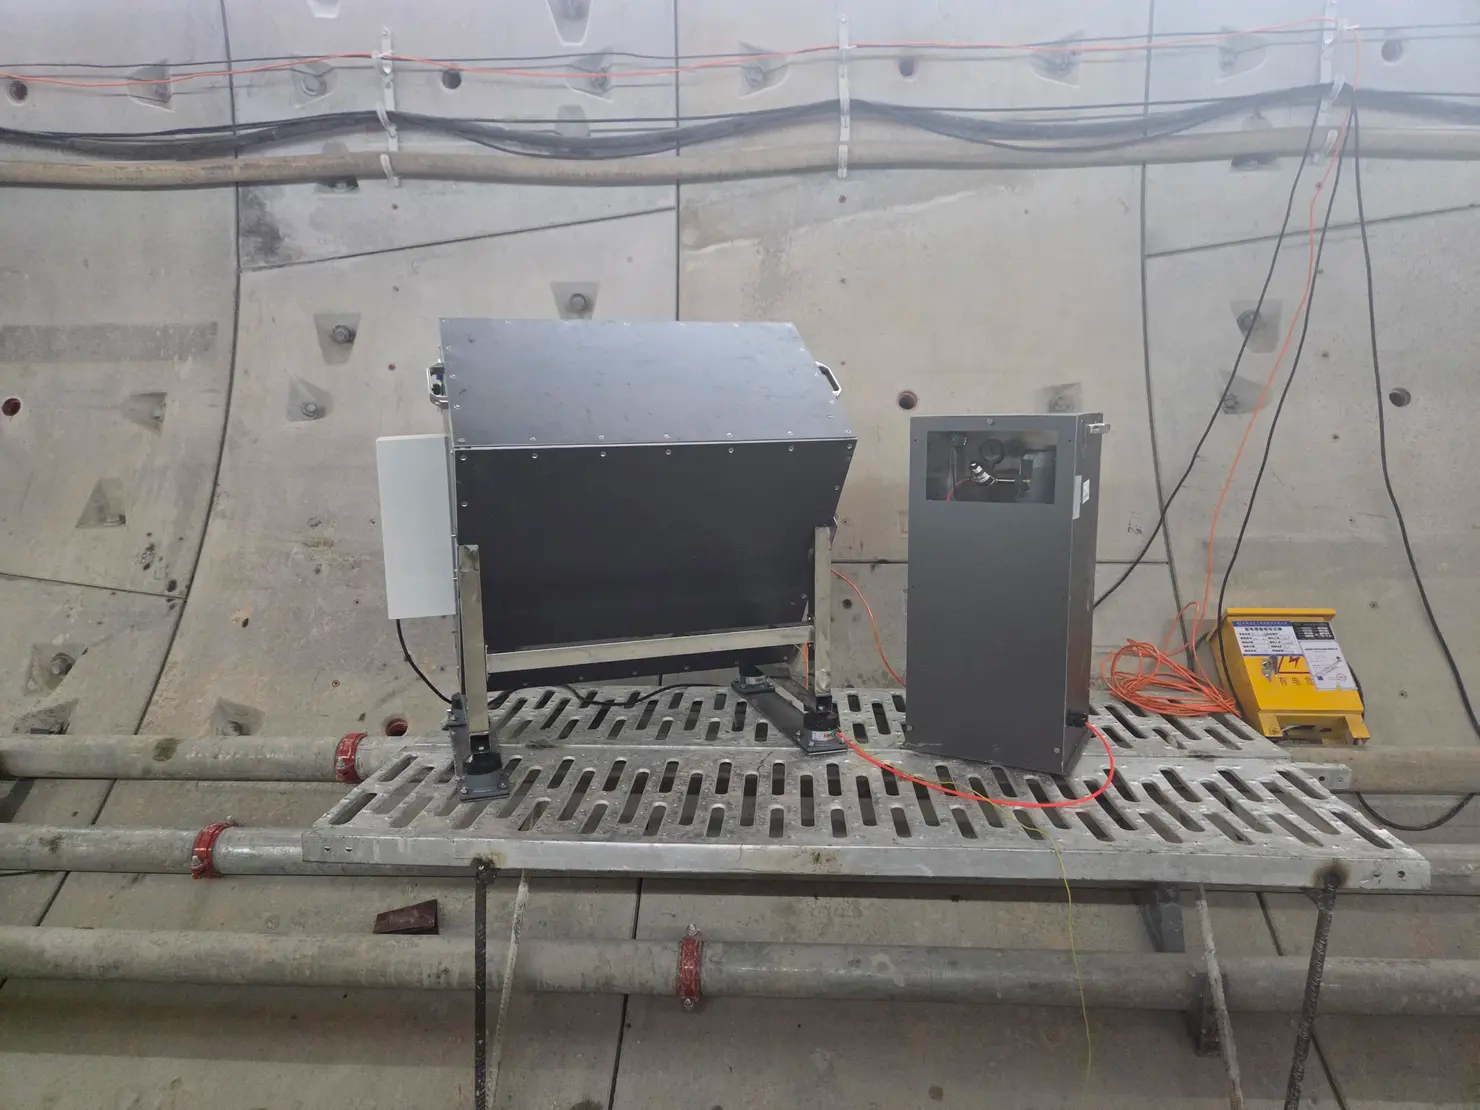
\includegraphics[width=0.244\textwidth]{pipeline_field_p1.png}};
\node[anchor=north west,inner sep=0] (C) at ([xshift=1mm]B.north east) {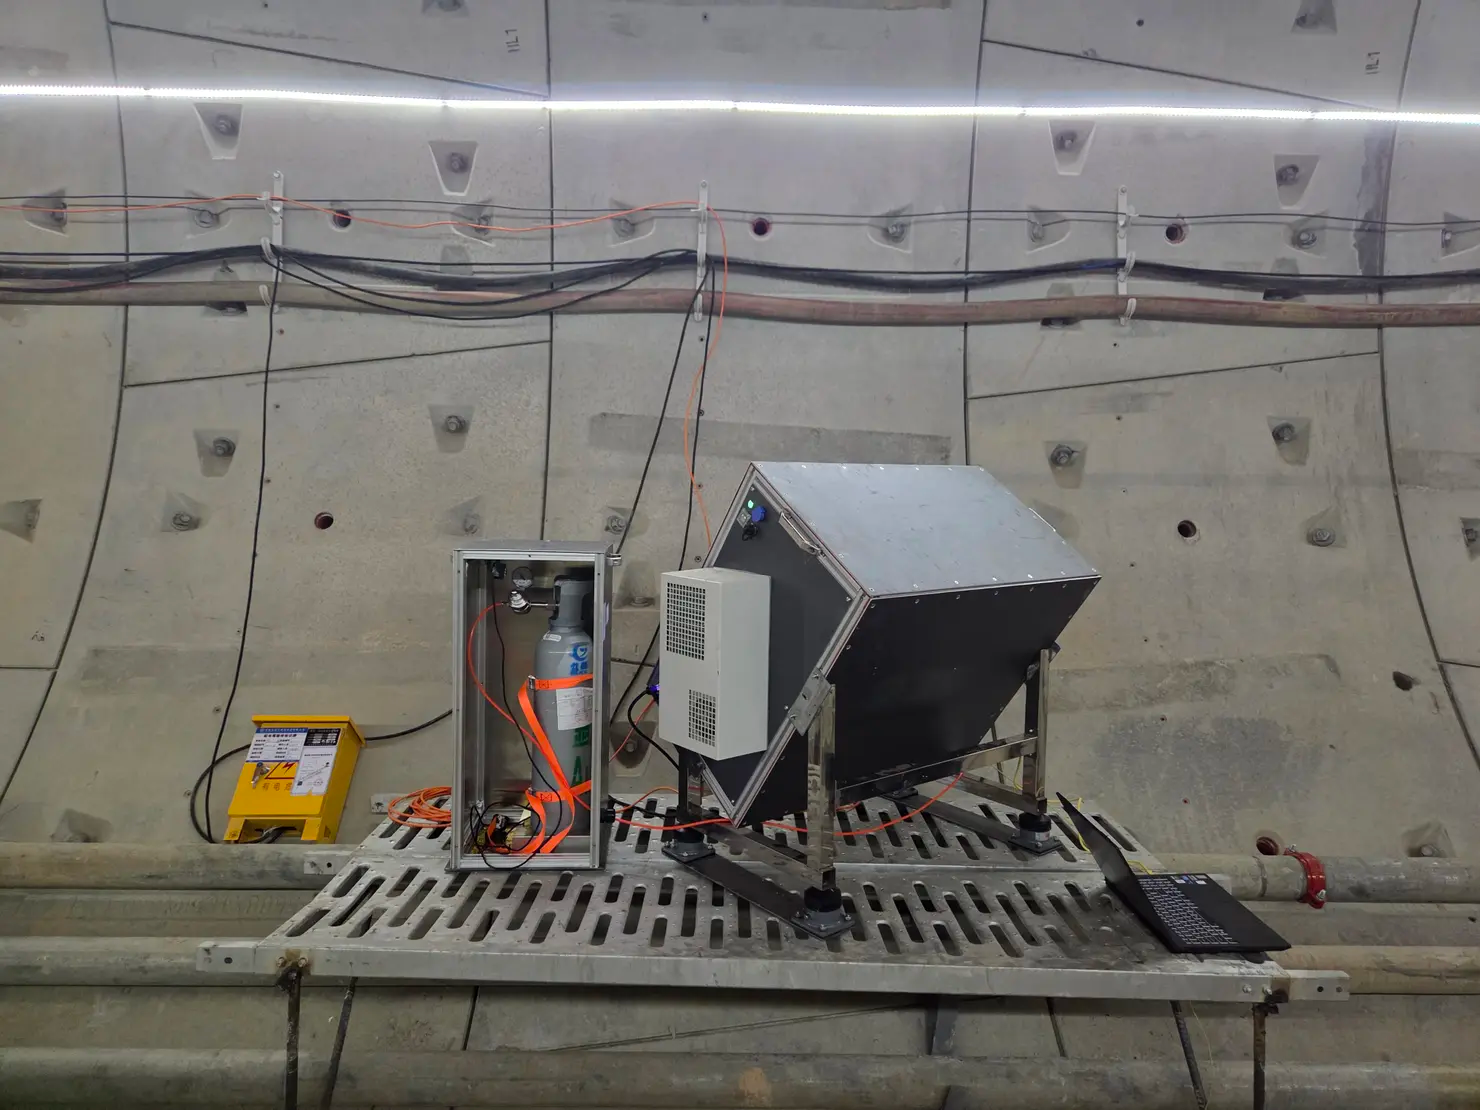
\includegraphics[width=0.244\textwidth]{pipeline_field_p2.png}};
\node[anchor=north west,inner sep=0] (D) at ([xshift=1mm]C.north east) {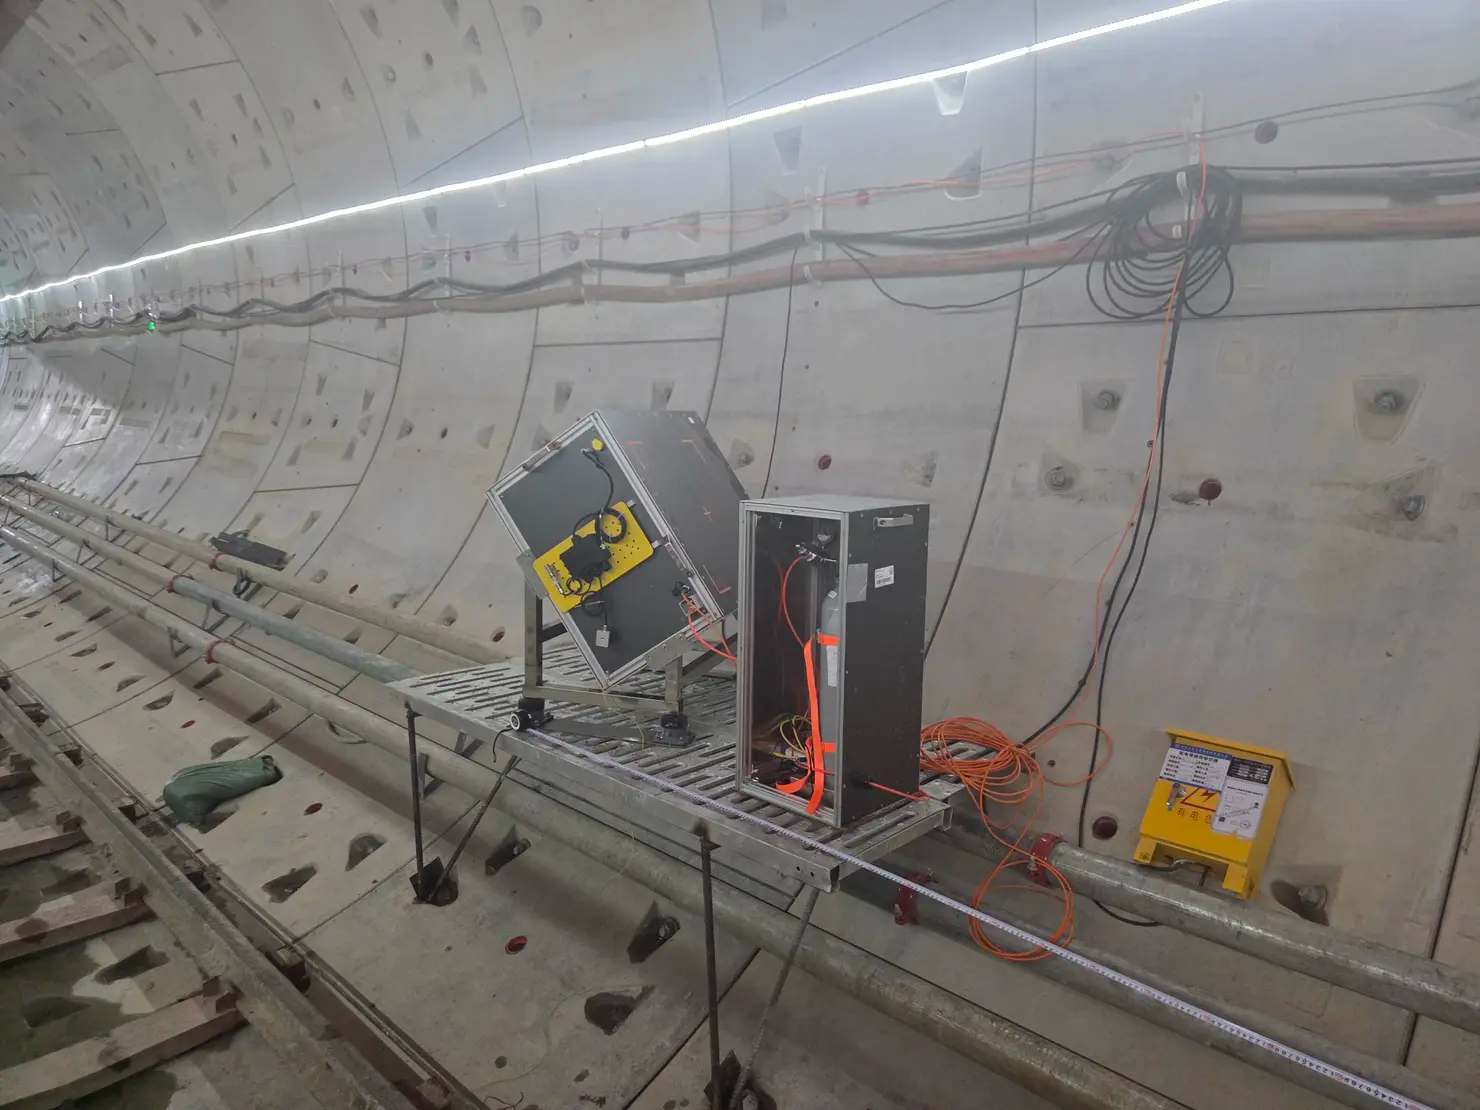
\includegraphics[width=0.244\textwidth]{pipeline_field_p3.png}};
\foreach \panel/\letter in {A/a,B/b,C/c,D/d}{
\node[anchor=north west,fill=white,fill opacity=0.72,text opacity=1,
      inner xsep=3pt,inner ysep=2pt,font=\bfseries\fontsize{9}{10}\selectfont]
      at ([xshift=0.5mm,yshift=-0.5mm]\panel.north west) {(\letter)};
}
\end{tikzpicture}
\caption{Field deployment for the pipeline survey at (a) P0, (b) P1, (c) P2 and (d) P3.}
\label{fig:pipeline-deployment}
\end{figure}


\subsection{Algorithm design}
The workflow separated feature detection from three-dimensional localisation. First, a position-specific U-Net \autocite{ronneberger2015} was trained on simulated directional maps containing pipelines with varied locations and orientations, together with cases containing no pipeline. Each network converted its field map into relative feature scores, which indicate pipeline-like structure but are not calibrated probabilities. Evaluation on 50,000 simulated test samples per position gave pixel ROC-AUC values of 0.9585--0.9703. As shown in Figure~\ref{fig:ridges}, all four field score maps contained an extended ridge.

\begin{figure}[htbp]
\centering
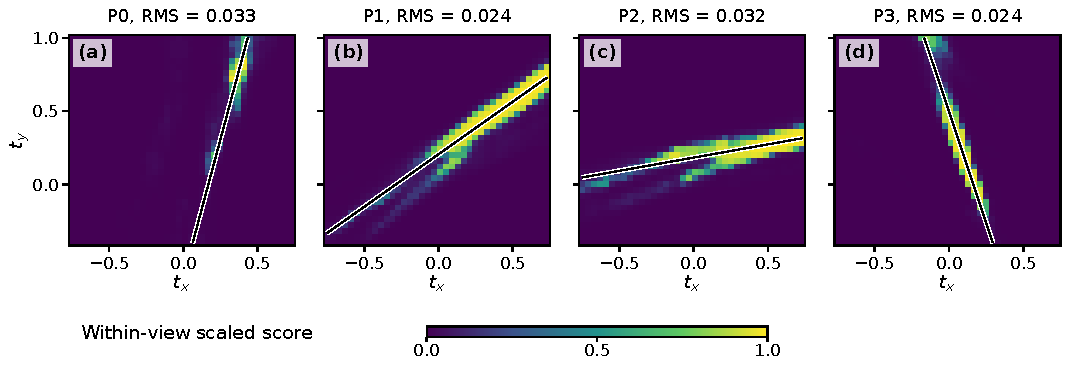
\includegraphics[width=\textwidth]{figure5_pipeline_projected_ridges.pdf}
\caption{Pipeline directional maps at (a) P0, (b) P1, (c) P2 and (d) P3. Colours represent within-view scaled network scores; lines mark fitted ridges. Coordinates are detector-local slopes; RMS denotes the weighted root-mean-square residual transverse to each ridge.}
\label{fig:ridges}
\end{figure}

A weighted straight ridge was then fitted to the high-score region in each map, and the measured detector poses transformed the ridges into backprojection planes in the tunnel frame. The candidate axis is the line most consistent with all four planes, with empirical view weights based on ridge linearity and residual, and a soft preference for a near-horizontal direction reflecting the expected utility geometry.

\subsection{Candidate axis and engineering use}
The fitted candidate axis (Figure~\ref{fig:axis}) crosses above the tunnel centreline at $X\approx-3.8$~m and $Z\approx6.5$~m, about 3.4~m above the lining extrados and 10.3~m below ground. It trends at about $47^\circ$ to the tunnel axis and is nearly horizontal (dip about $3^\circ$).

\begin{figure}[htbp]
\centering
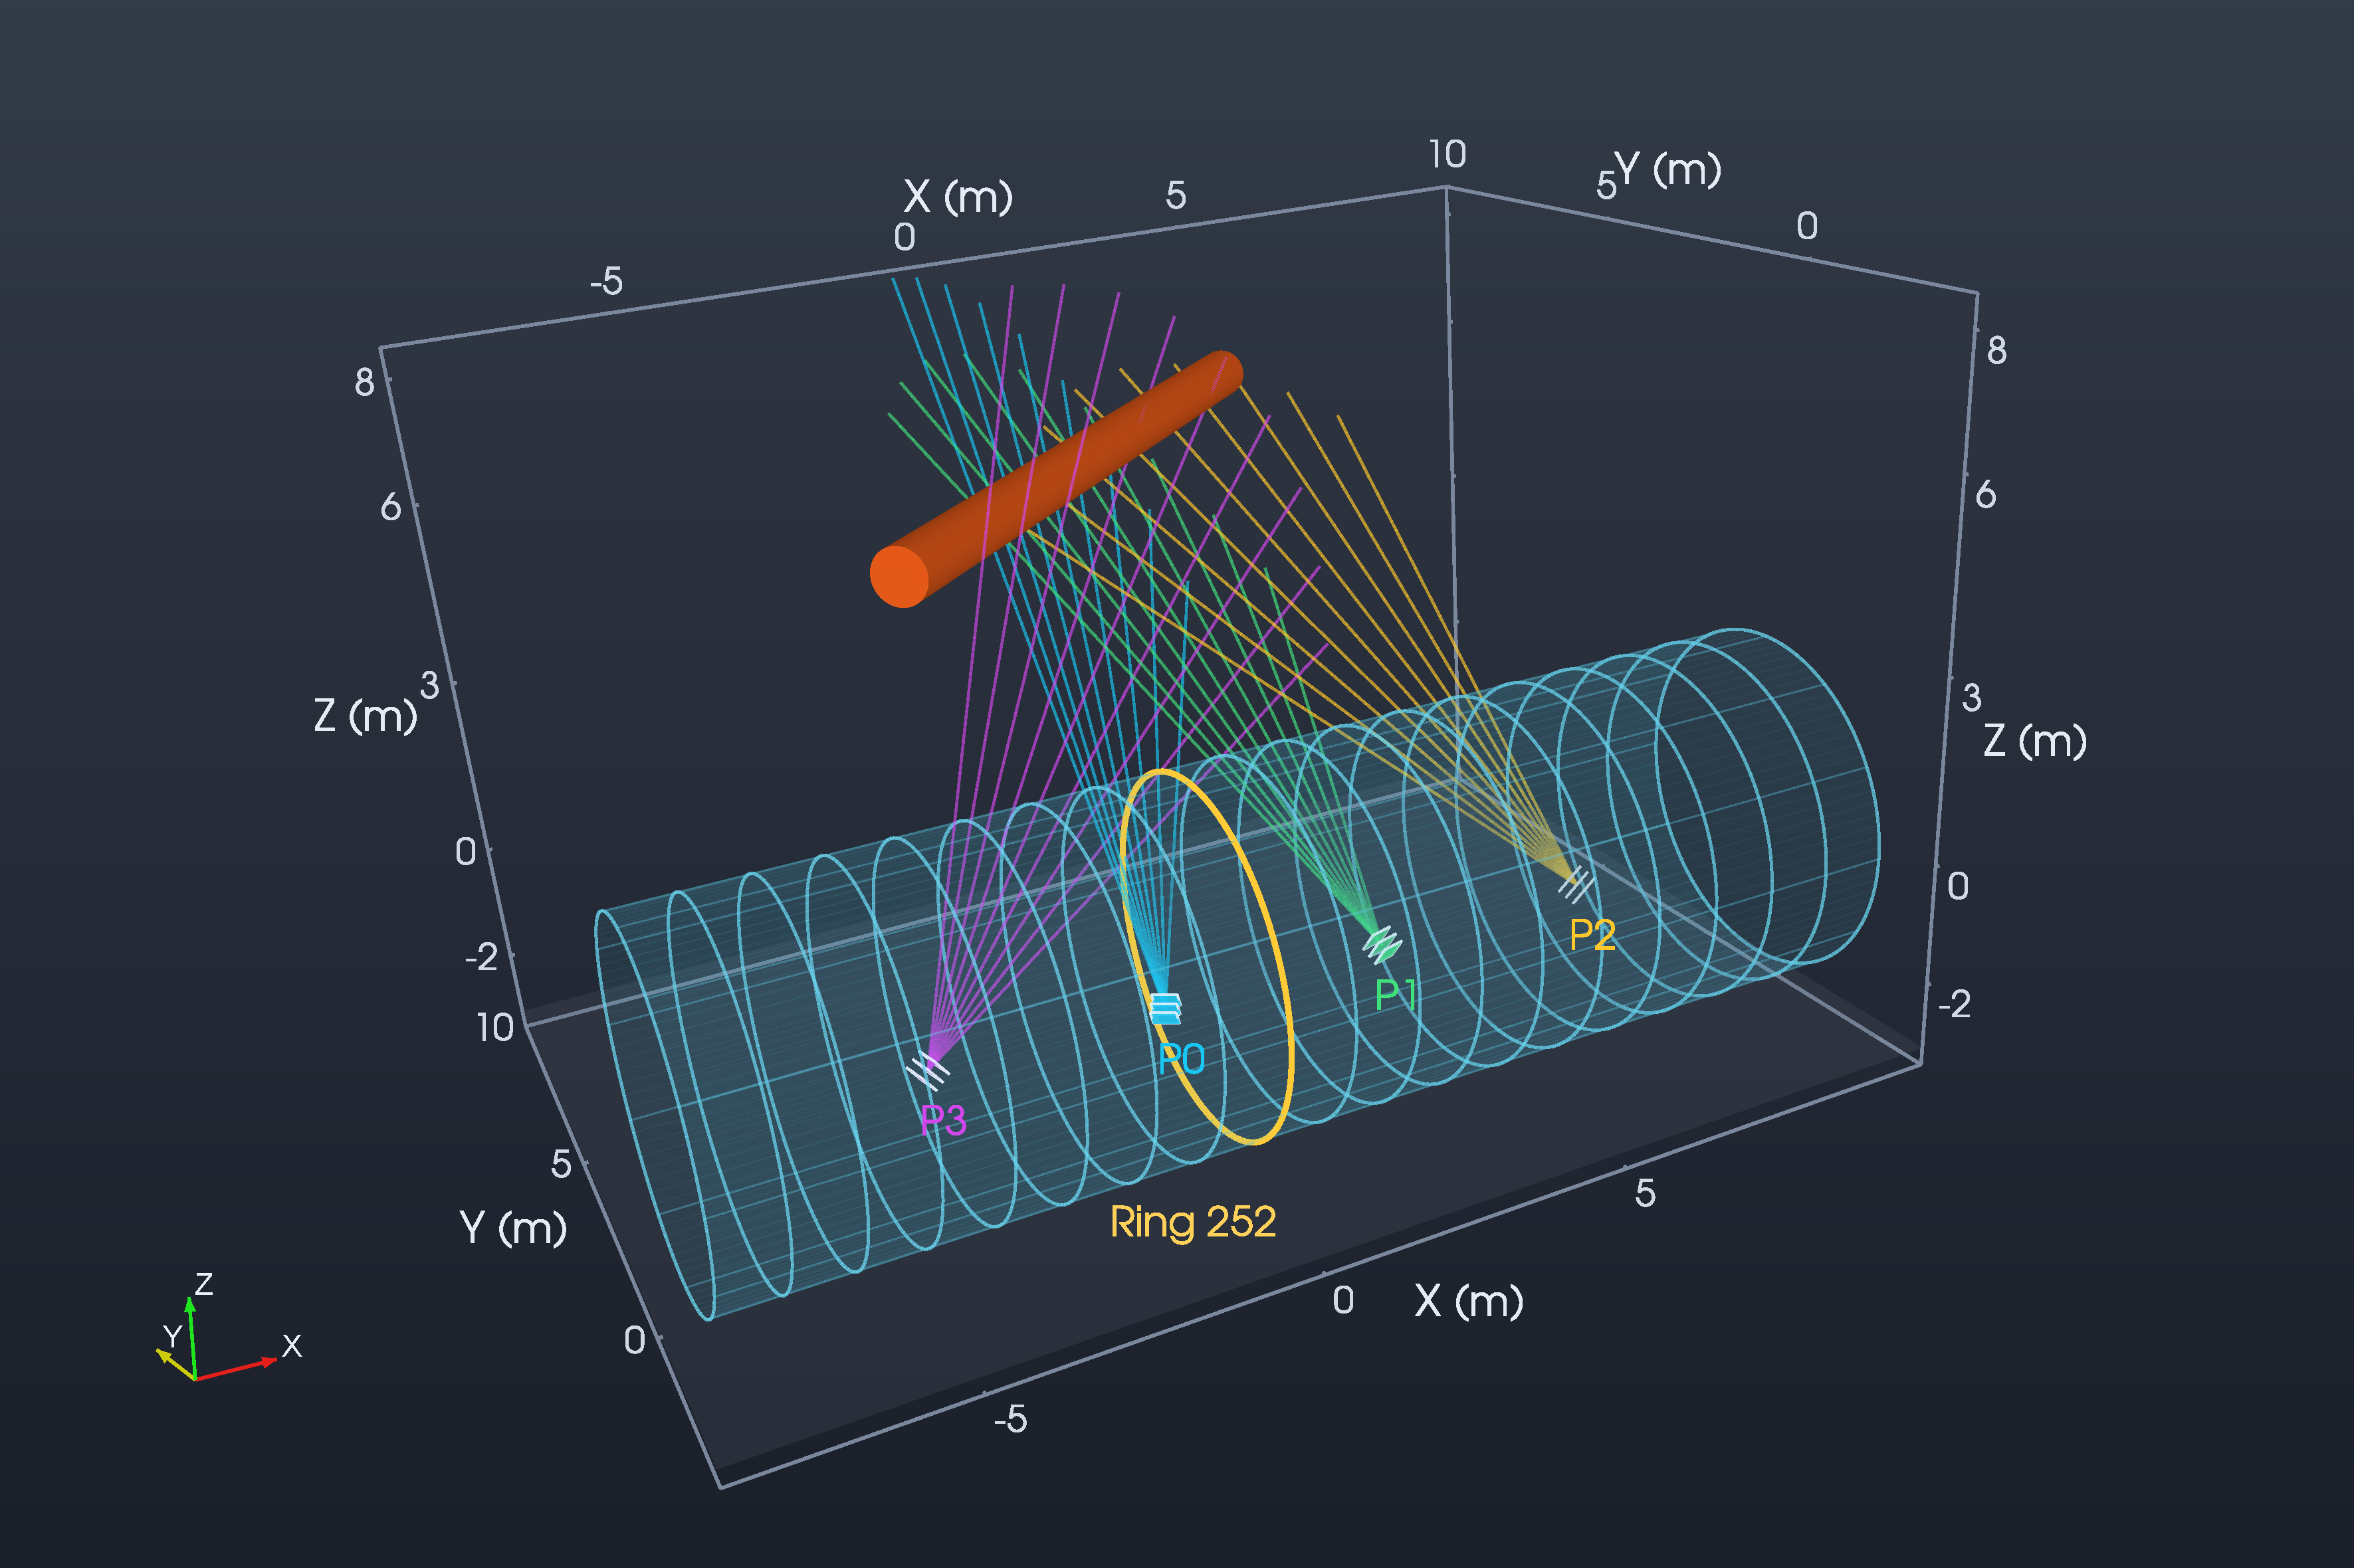
\includegraphics[width=0.56\textwidth]{figure6_pipeline_axis_horizontal.pdf}
\caption{Three-dimensional pipeline candidate axis with the horizontal soft constraint. Coloured ray fans represent the backprojection planes from P0--P3; the orange tube shows the candidate pipe with its reported diameter of 0.8~m.}
\label{fig:axis}
\end{figure}

The candidate position and shield-avoidance recommendations were supplied to the construction team as precautionary spatial information. The team reported implementing avoidance measures based on this information.

\subsection{Limitations}
The line is a candidate axis, not independent confirmation. The networks were evaluated on simulated data and their field outputs are not calibrated probabilities. The axis also depends on detector poses, empirical weights and the horizontal penalty; no positional uncertainty or independent confirmation was available.

\section{DISCUSSION}
\subsection{Instrumentation lessons}
The campaign shows that one transportable Micromegas system can support dynamic TBM-mounted and stationary multi-position measurements. Pneumatic isolation kept TBM vibration from the detectors, and the low-consumption gas supply allowed about three months between routine services. Most right-line downtime arose from external power and network interruptions, making site infrastructure part of the deployment design.

\subsection{Use in construction decision-making}
Figure~\ref{fig:workflow} summarises how the two demonstrations moved from field measurement to an engineering decision. Both shared the same measurement chain, from defining the engineering question and measurement geometry to quality-controlled directional maps, but used different interpretation branches: a physics-based inversion against the borehole model for ground density, and learned feature detection combined with multi-view geometry for the pipeline. Neither output was treated as confirmation. Each passed through an evidence review of consistency, reference compatibility and pose sensitivity before informing a precautionary decision, and unresolved uncertainty can direct further measurement positions.

Acquisition required approximately 21--34~h per position, while the right-line drive averaged about 6.5 rings per day. The present system is therefore better suited to targeted screening of known concerns, such as a suspected utility crossing or a section with sparse borehole control, than to continuous warning ahead of the face. Its results should be combined with boreholes, construction geometry and conventional investigations. Quantitative interpretation remains limited by reference compatibility, sparse viewpoints and unquantified uncertainty; future work should use matched sky references, systematic pose records, additional views, sensitivity studies and independently confirmed targets.

\begin{figure}[htbp]
\centering
\resizebox{0.66\textwidth}{!}{%
\begin{tikzpicture}[
  font=\sffamily\small,
  >=Latex,
  box/.style={draw=wfink, rounded corners=2pt, line width=0.55pt,
    align=center, minimum height=11mm, inner sep=4pt},
  field/.style={box, fill=wffield, text width=39mm},
  density/.style={box, fill=wfdensity, text width=58mm},
  pipeline/.style={box, fill=wfpipeline, text width=58mm},
  decision/.style={box, fill=wfdecision, text width=46mm},
  check/.style={box, fill=wfcheck, text width=78mm, font=\sffamily\footnotesize},
  arrow/.style={-{Latex[length=2.3mm]}, line width=0.75pt, draw=wfink},
  feedback/.style={-{Latex[length=2.3mm]}, dashed, line width=0.7pt, draw=wfink}
]
\node[field] (plan) {Define engineering question\\and measurement geometry};
\node[field, right=7mm of plan] (measure) {Acquire tracks and\\record detector poses};
\node[field, right=7mm of measure] (map) {Build quality-controlled\\directional muon maps};
\draw[arrow] (plan) -- (measure);
\draw[arrow] (measure) -- (map);
\node[density, below left=18mm and -14mm of measure] (density)
  {\textbf{Density imaging (Demonstration I)}\\Compare counts with a borehole-based transmission model; estimate regularised 3D corrections};
\node[pipeline, below right=18mm and -14mm of measure] (pipeline)
  {\textbf{Pipeline localisation (Demonstration II)}\\Detect pipeline-like features with simulation-trained networks; combine ridges using multi-view geometry};
\node[decision, below=6mm of density] (screen) {Possible density anomaly\\for geological screening};
\node[decision, below=6mm of pipeline] (axis) {Candidate pipeline axis\\for avoidance planning};
\node[check, below=15mm of $(screen)!0.5!(axis)$] (review)
  {\textbf{Evidence review}\\Consistency checks, reference compatibility, pose sensitivity and independent confirmation where available};
\node[decision, below=6mm of review, text width=48mm] (action)
  {Precautionary\\engineering decision};
\draw[arrow] (map.south) -- ++(0,-5mm) -| (density.north);
\draw[arrow] (map.south) -- ++(0,-5mm) -| (pipeline.north);
\draw[arrow] (density) -- (screen);
\draw[arrow] (pipeline) -- (axis);
\draw[arrow] (screen.south) -- ++(0,-4mm) -| (review.north);
\draw[arrow] (axis.south) -- ++(0,-4mm) -| (review.north);
\draw[arrow] (review) -- (action);
\coordinate (fb1) at ([xshift=-18mm]density.west |- review.west);
\coordinate (fb2) at (fb1 |- plan.west);
\draw[feedback] (review.west) -- (fb1) -- (fb2) -- (plan.west);
\node[font=\sffamily\footnotesize, rotate=90, anchor=south]
  at ($(fb1)!0.5!(fb2)$) {Uncertainty may guide additional measurements};
\end{tikzpicture}%
}
\caption{Field-to-decision workflow for tunnel muography. Both demonstrations share the measurement chain and differ in interpretation; each output is reviewed before it informs a precautionary engineering decision.}
\label{fig:workflow}
\end{figure}


\section{CONCLUSIONS}
A three-layer Micromegas system completed sustained field deployment on Shenzhen Metro Line~22. Right-line acquisition availability was 85.2\% overall and 97.2\% after external interruptions were excluded, and platform vibration during TBM operation was not detected inside the isolated enclosure. Dynamic measurements indicated a possible low-density region relative to the borehole model, and a static four-position investigation produced a candidate pipeline axis for avoidance planning. These results establish field feasibility and decision-support potential, but require improved reference measurements, additional viewpoints, uncertainty quantification and independent validation.

\section*{ACKNOWLEDGEMENTS}
The authors acknowledge Shenzhen Metro Group Co., Ltd. for field access and coordination, the University of Science and Technology of China for research support, the Jianwei teams for equipment and maintenance, and the site personnel for assistance with installation and data acquisition.

\section*{REFERENCES}
\printbibliography[heading=none]
\end{document}
